\chapter{Anhang}

	\section{Klassendiagramm}
	
	
%	\getlength{\paperwidth}\\
%	\getlength{\paperheight}\\
%	\getlength{\pdfpageheight}\\
%	\getlength{\pdfpagewidth}\\
%	\getlength{\headwidth}\\
%	\getlength{\footskip}\\
%	\getlength{\textwidth}\\
%	\getlength{\textheight}\\
%	\getlength{\vsize}\\
%	\getlength{\hsize}\\
	
	\newpage
		
	\paperwidth=4.5\pdfpageheight
	\paperheight=4.5\pdfpagewidth
	\pdfpageheight=\paperheight
	\pdfpagewidth=\paperwidth
	%\addtolength{\textheight}{1cm}
	\headwidth=1.05\textheight
	
	\begingroup 
	\vsize=\textwidth
	\hsize=1.05\textheight
	
	\textwidth=\hsize
	\textheight=\vsize
		
		
	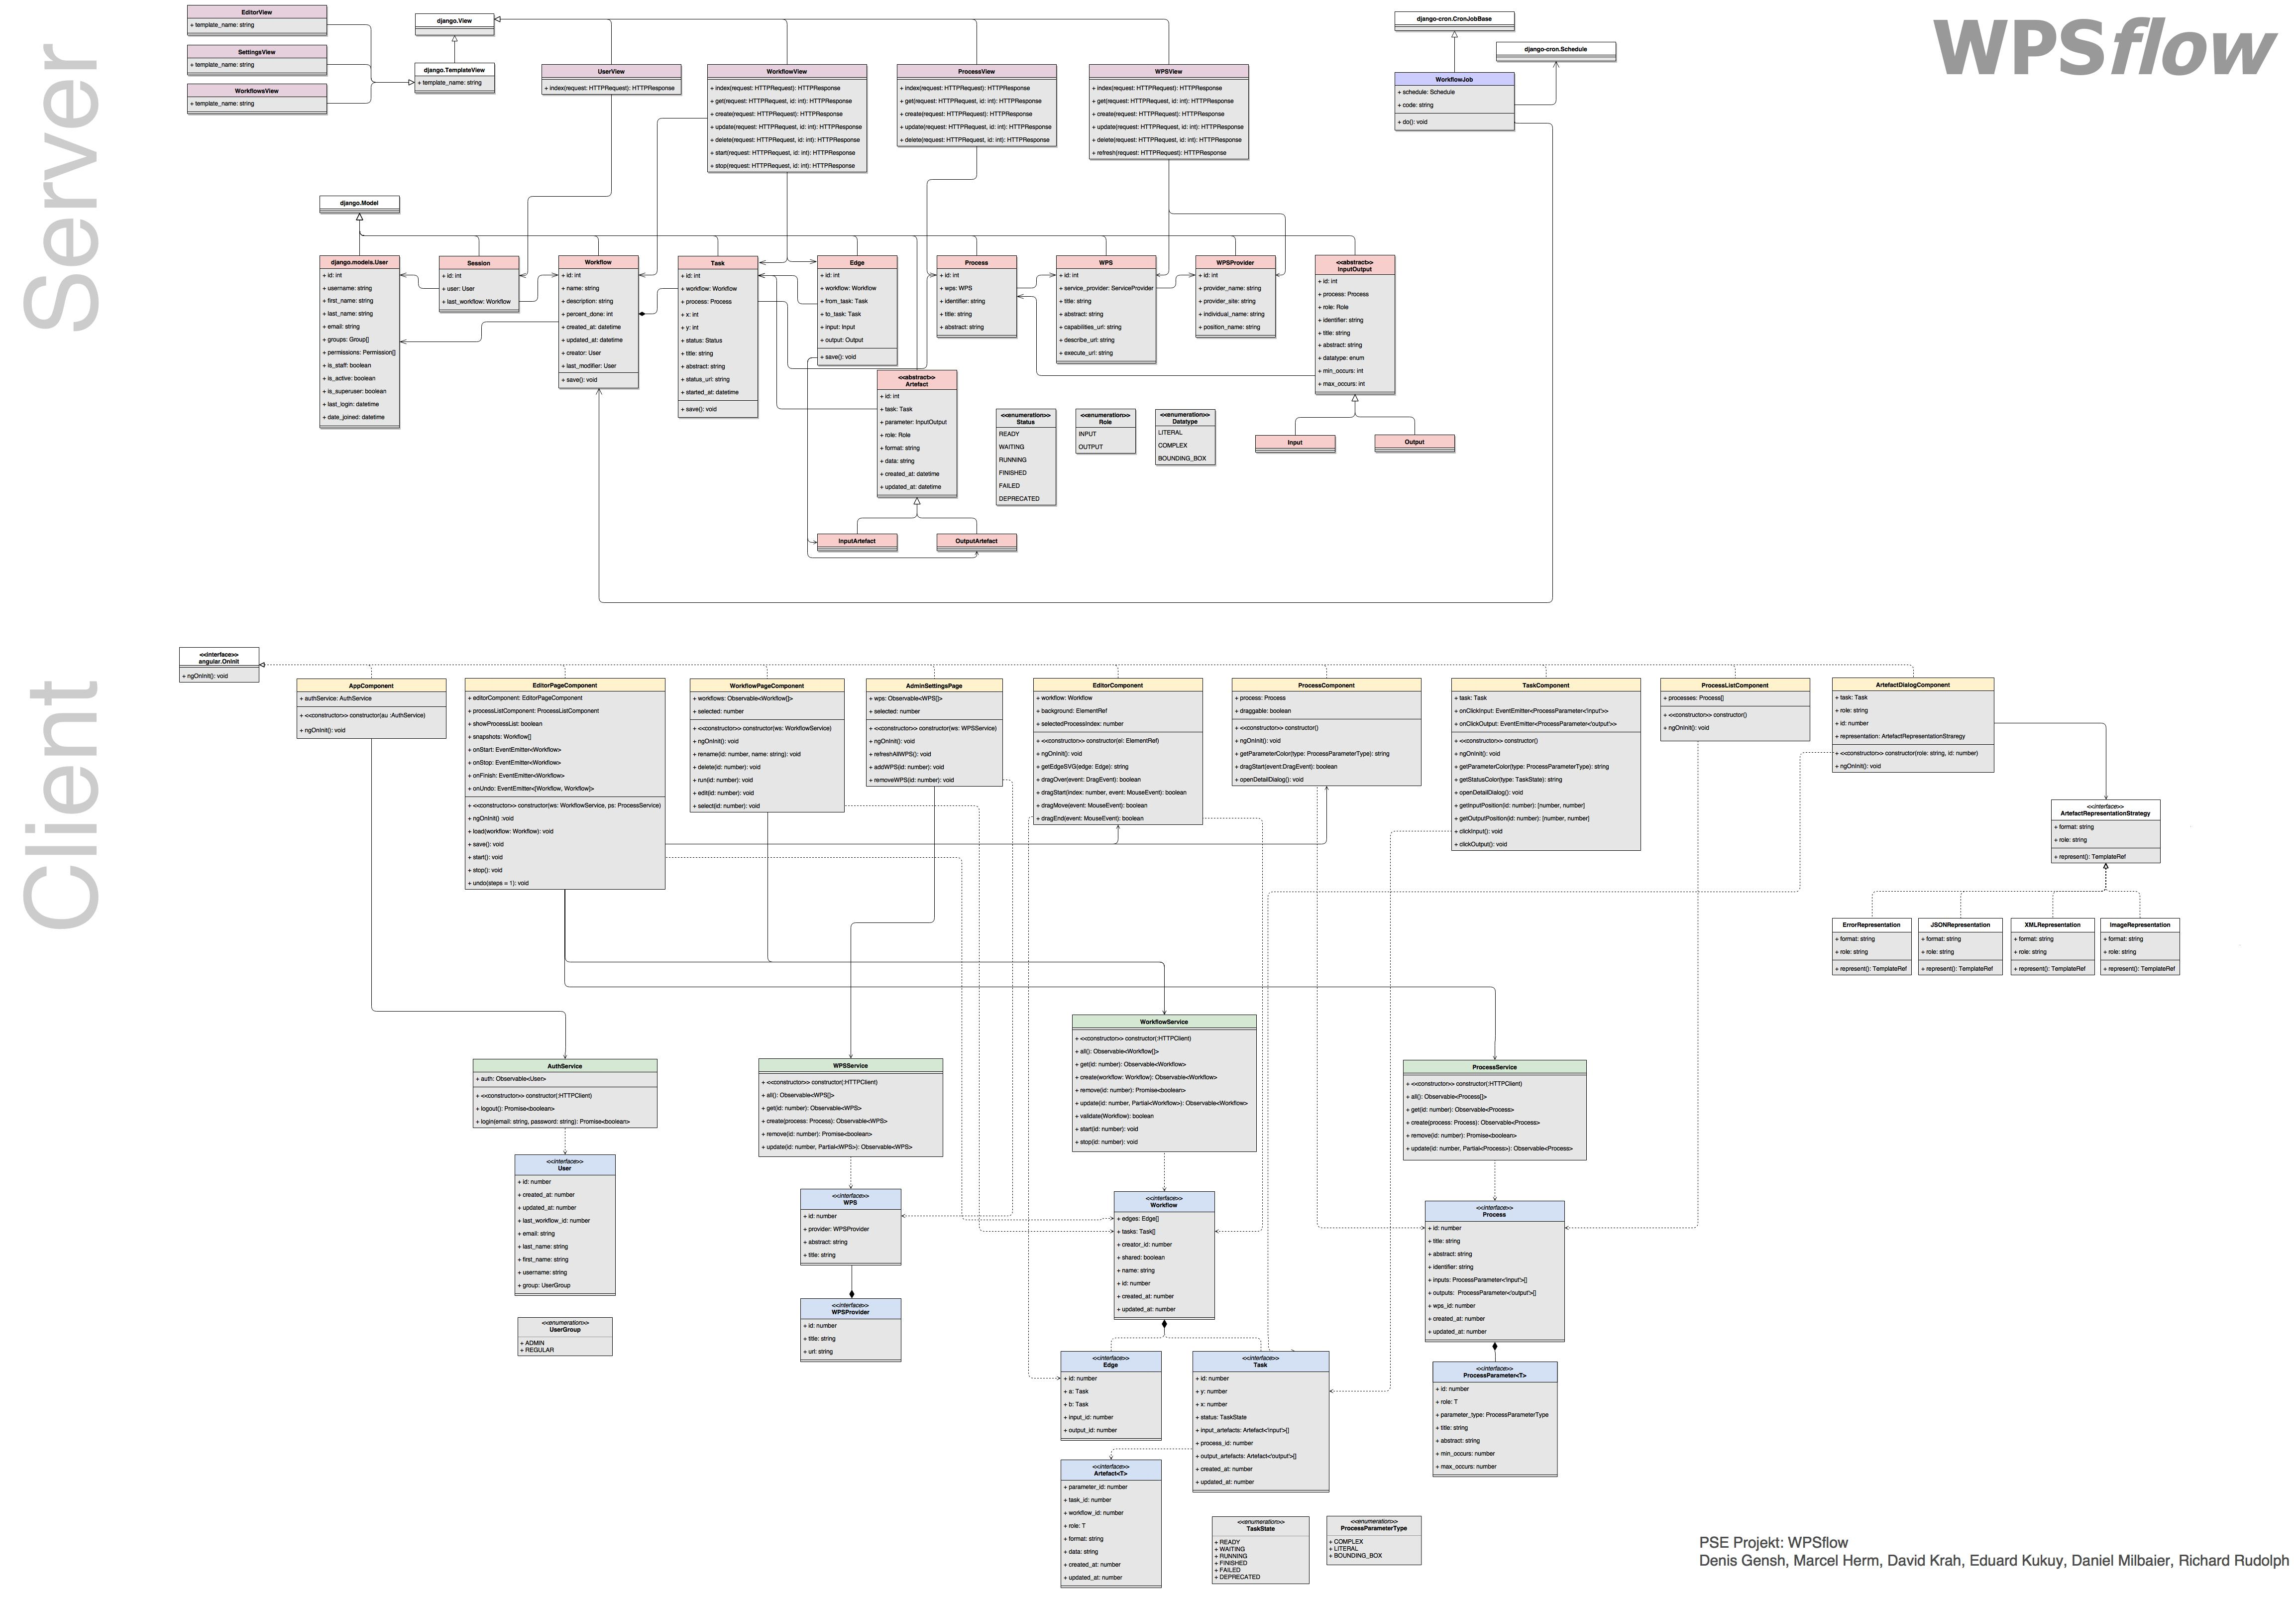
\includegraphics[width=\pdfpagewidth-3cm]{diagrams/class-diagram-complete.jpg}
%	\includesvg{diagrams/class-diagram-complete.svg}	

	
	
	
    \endgroup
	\newpage
	\paperwidth=\pdfpageheight
	\paperheight=\pdfpagewidth
	\pdfpageheight=\paperheight
	\pdfpagewidth=\paperwidth
	\headwidth=\textwidth
	
	%\section{test}
%	\getlength{\paperwidth}\\
%	\getlength{\paperheight}\\
%	\getlength{\pdfpageheight}\\
%	\getlength{\pdfpagewidth}\\
%	\getlength{\headwidth}\\
%	\getlength{\footskip}\\
%	\getlength{\textwidth}\\
%	\getlength{\textheight}\\
%	\getlength{\vsize}\\
%	\getlength{\hsize}\\